\begin{figure}[t]
    \centering
    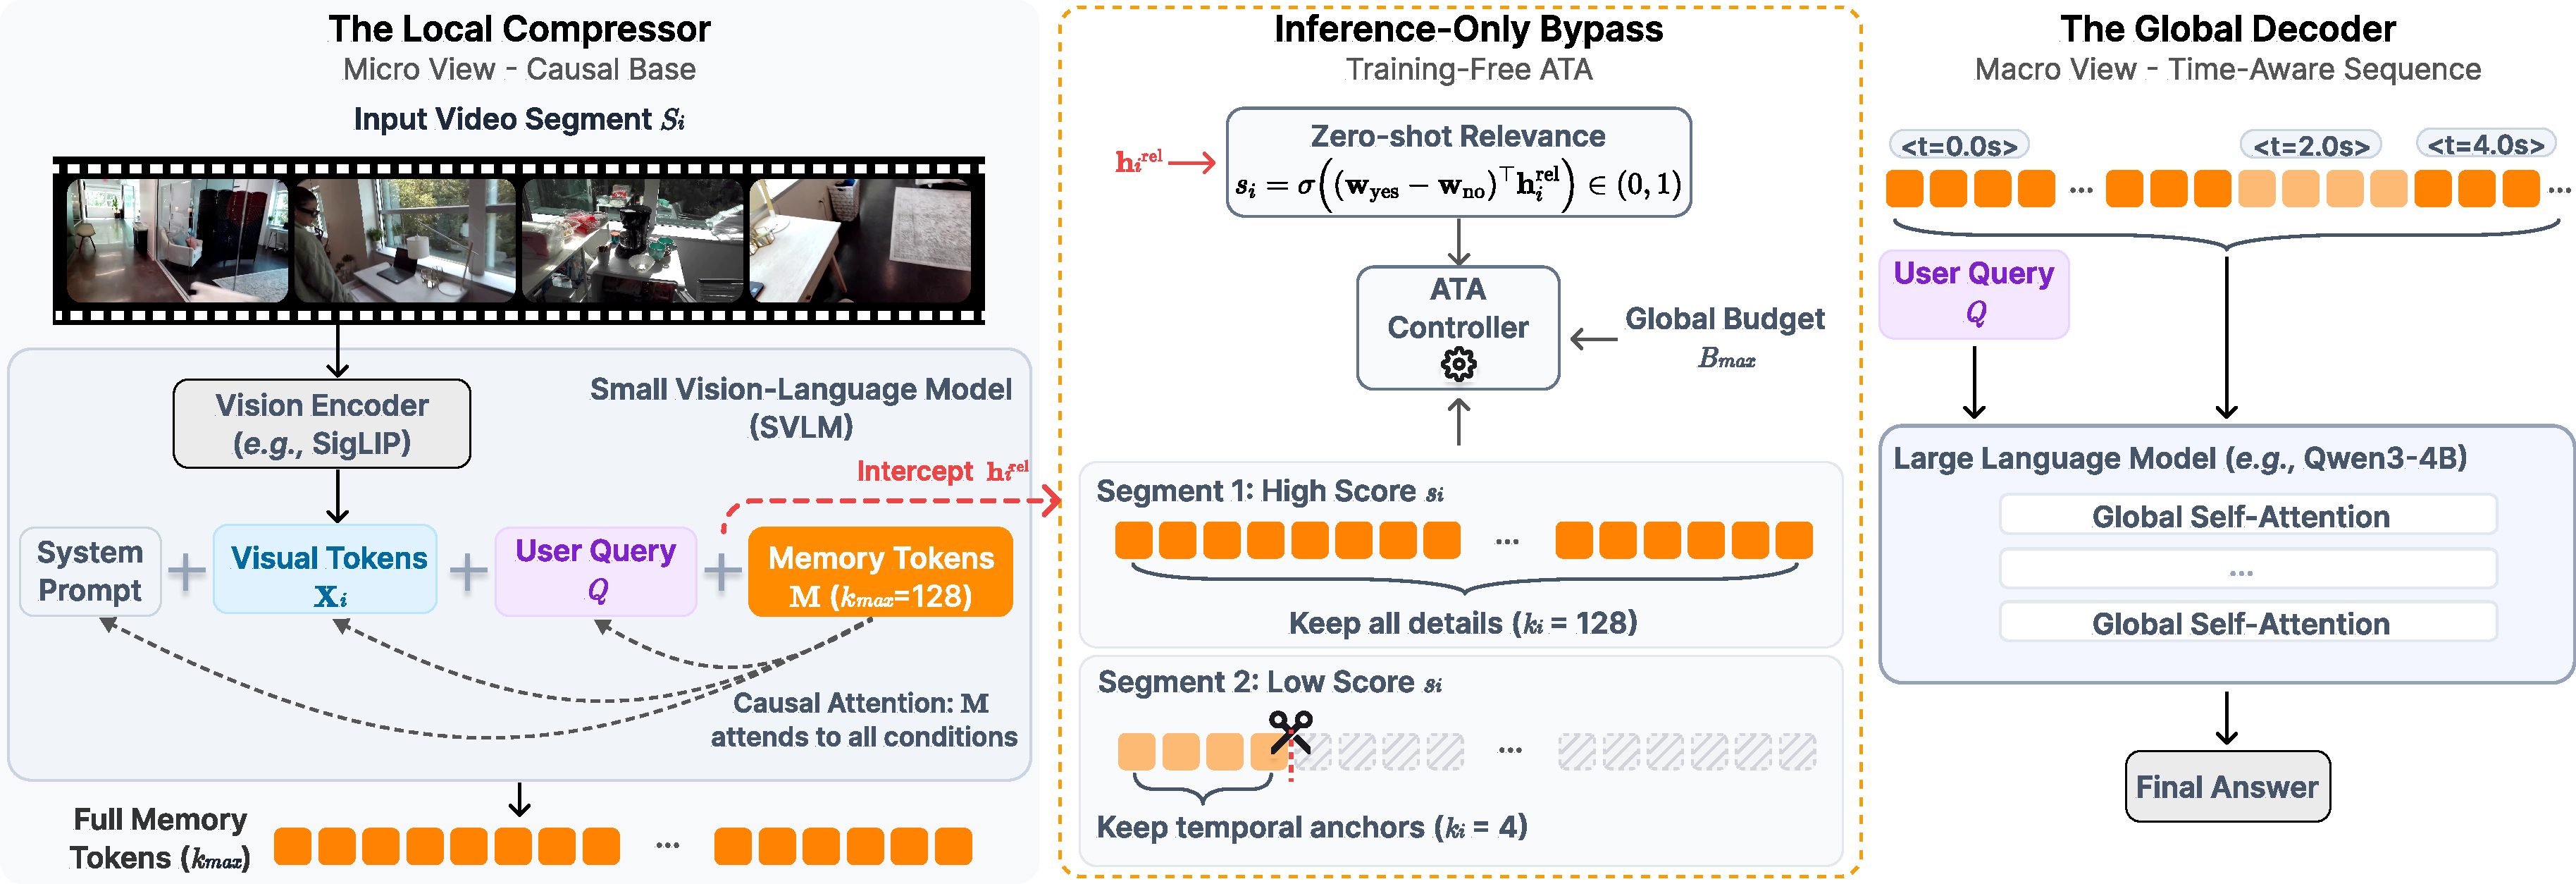
\includegraphics[width=\textwidth]{fig/tempo.pdf}
    \caption{
        \textbf{Overview of the Tempo framework.} 
        Our unified architecture casts long video understanding as an end-to-end, query-aware compression process. 
        \textbf{The Local Compressor (Left).} For each segment, a Small Vision-Language Model (SVLM) acts as a semantic temporal compressor. Under causal attention, learnable memory tokens $\mathbf{M}$ inherently distill the preceding visual tokens $\mathbf{X}_i$ and user query $Q$. 
        \textbf{Inference-Only Bypass (Middle).} During a single forward pass, an Adaptive Token Allocation (ATA) controller intercepts the hidden state $\mathbf{h}_i^{\mathrm{rel}}$ to compute a zero-shot relevance score $s_i$. This enables an $\mathcal{O}(1)$ dynamic head truncation, allocating dense bandwidth to query-critical segments while compressing redundancies into minimal temporal anchors to strictly satisfy a global budget $B_{\max}$. 
        \textbf{The Global Decoder (Right).} The compressed memory tokens are assembled into a highly sparse, time-aware sequence using explicit temporal tags (\eg, \texttt{<t=2.0s>}). A global LLM synthesizes this condensed multimodal context to generate the final response.
    }
    % \vspace{-0.8em}
    \label{fig:tempo}
\end{figure}
